%Preamble
\documentclass[12pt]{article}
\usepackage{fancyhdr}
\usepackage{extramarks}
\usepackage{amsmath}
\usepackage{amssymb}
\usepackage{amsthm}
\usepackage{amsrefs}
\usepackage{amsfonts}
\usepackage{mathrsfs}
\usepackage{mathtools}
\usepackage[mathcal]{eucal} %% changes meaning of \mathcal
\usepackage{enumerate}
\usepackage[shortlabels]{enumitem}
\usepackage{verbatim} %% includes comment environment
\usepackage{hyperref}
\usepackage[capitalize]{cleveref}
\crefformat{equation}{~(#2#1#3)}
\usepackage{caption, subcaption}
\usepackage{graphicx}
\usepackage{fullpage} %%smaller margins
\usepackage[all,arc]{xy}
\usepackage{mathrsfs}

\hypersetup{
    linktoc=all,     % set to all if you want both sections and subsections linked
}

\topmargin=-0.45in
\evensidemargin=0in
\oddsidemargin=0in
\textwidth=6.5in
\textheight=9.0in
\headsep=0.25in
\setlength{\headheight}{16pt}

\linespread{1.0}

\pagestyle{fancy}
\lhead{\Name}
\chead{\hwClass: \hwTitle}
\rhead{\hwDueDate}
\lfoot{\lastxmark}
\cfoot{\thepage}

\renewcommand\headrulewidth{0.4pt}
\renewcommand\footrulewidth{0.4pt}

\setlength\parindent{0pt}

%% Title Info
\newcommand{\hwTitle}{HW \# 5}
\newcommand{\hwDueDate}{Feb 26, 2021}
\newcommand{\hwClass}{AMATH 568}
\newcommand{\hwClassTime}{}
\newcommand{\hwClassInstructor}{}
\newcommand{\Name}{\textbf{Marlin Figgins}}


%% MATH MACROS
\newcommand{\bbF}{\mathbb{F}}
\newcommand{\bbN}{\mathbb{N}}
\newcommand{\bbQ}{\mathbb{Q}}
\newcommand{\bbR}{\mathbb{R}}
\newcommand{\bbZ}{\mathbb{Z}}
\newcommand{\bbC}{\mathbb{C}}
\newcommand{\abs}[1]{ \left| #1 \right| }
\newcommand{\diff}[2]{\frac{d #1}{d #2}}
\newcommand{\infsum}[1]{\sum_{#1}^{\infty}}
\newcommand{\norm}[1]{ \left|\left| #1 \right|\right| }
\newcommand{\eval}[1]{ \left. #1 \right| }
\newcommand{\Expect}[1]{\mathbb{E}\left[#1 \right]}
\newcommand{\Var}[1]{\mathbb{V}\left[#1 \right]}
\renewcommand{\vec}[1]{\mathbf{#1}}

\renewcommand{\phi}{\varphi}
\renewcommand{\emptyset}{\O}

%--------Theorem Environments--------
%theoremstyle{plain} --- defaultx
\newtheorem{thm}{Theorem}[section]
\newtheorem{cor}[thm]{Corollary}
\newtheorem{prop}[thm]{Proposition}
\newtheorem{lem}[thm]{Lemma}
\newtheorem{conj}[thm]{Conjecture}
\newtheorem{quest}[thm]{Question}

\theoremstyle{definition}
\newtheorem{defn}[thm]{Definition}
\newtheorem{defns}[thm]{Definitions}
\newtheorem{con}[thm]{Construction}
\newtheorem{exmp}[thm]{Example}
\newtheorem{exmps}[thm]{Examples}
\newtheorem{notn}[thm]{Notation}
\newtheorem{notns}[thm]{Notations}
\newtheorem{addm}[thm]{Addendum}

% Environments for answers and solutions
\newtheorem{exer}{Exercise}
\newtheorem{sol}{Solution}

\theoremstyle{remark}
\newtheorem{rem}[thm]{Remark}
\newtheorem{rems}[thm]{Remarks}
\newtheorem{warn}[thm]{Warning}
\newtheorem{sch}[thm]{Scholium}

\makeatletter
\let\c@equation\c@thm
\makeatother

\begin{document}

\begin{exer}

Consider the singular equation:
\begin{equation*}
    \epsilon \frac{d^{2} u}{dx^{2}} + (1 + x)^{2} \frac{d u}{d x} + u = 0
\end{equation*}
with $u(0) = u(1) = 1$ and with $0 < \epsilon \ll 1$.
\begin{enumerate}[(a)]
    \item Obtain a uniform approximation which is valid to $O(\epsilon)$ i.e. determine the leading order behavior and first correction.
    \item Show that assuming the boundary layer to be at $x = 1$ is inconsistent. (Hint: Use the stretched inner varible  $\xi = (1 - x) / \epsilon$).
    \item Plot the uniform solution for $\epsilon = 0.01$, $0.05$,  $0.1$,  $0.2$.
\end{enumerate}
\end{exer}

\begin{sol}
    %TODO: Solve for leading order $u_{0}$ and its first correction $u_{1}$. Matching only occurs on $u_{0}$ to get uniform solution,

    (a) (Assuming this has a boundary layer at 0) We attempt the perturbation expansion which gives us terms

    %TODO: REDO THIS. x = \xi \epsilon 
    \begin{align*}
        O(1): &\quad (1 + x)^{2} u_{0x} + u_{0} = 0\\
        O(\epsilon): &\quad (1 + x)^{2} u_{1x} + u_{1} = -u_{0xx},
    \end{align*}
    for the outer problem this system only satisfies the right boundary condition i.e. $u(1)=1$. This gives us solution for the leading order as
     \begin{align*}
         u_{0}(x) = e^{\frac{1}{x+1} - \frac{1}{2}}.
    \end{align*}
    Computing the second derivative of this, we see that our $O(\epsilon)$ equation becomes
    \begin{align*}
        (1 + x)^{2} u_{1x} + u_{1} = - \frac{2x + 3}{(x+1)^{4}} e^{\frac{1}{x+1} - \frac{1}{2}}\\
        u_{1}(1) = 0.
    \end{align*}
    This has solution
    \begin{align*}
        u_{1}(x) &= c e^{\frac{1}{x+1}} + \left(\frac{x}{2}\right) \left( \frac{ e^{\frac{1}{x+1} - \frac{1}{2}}}{(x+1)^{5}}\right) +  \left(\frac{7}{10}\right) \left( \frac{ e^{\frac{1}{x+1} - \frac{1}{2}}}{(x+1)^{5}}\right)\\
        c &= - \frac{1}{2^{6}} \left( \frac{12}{5}\right) e^{-\frac{1}{2}}.
    \end{align*}
    
    We'll now tackle the inner problem using the coordinate transformation $\xi = \frac{x}{\epsilon}$. In these coordinates, our equation becomes
    \begin{align*}
        u_{\xi \xi} + (1 +  \epsilon\xi)^{2} u_{\xi} + \epsilon u = 0,\\
        u_{\xi \xi} + u_{\xi} + 2\epsilon \xi u_{\xi} + \epsilon^{2}\xi^{2} u_{\xi} + \epsilon u = 0
    \end{align*}
    with bondary condition  $u(\epsilon \xi = 0) = 1$. Now doing a pertubation expansion, we see that
    \begin{align*}
        O(1):  &\quad u_{0\xi \xi} + u_{0\xi} = 0\\
        O(\epsilon): &\quad u_{1\xi \xi} + u_{1\xi} = - u_{0} - 2 \xi u_{0\xi}
    \end{align*}
    with boundary conditions $u_{0}(\xi = 0) = 1$ and $u_{1}(\xi = 0) = 0$. The leading order solution in this case is then given by
    \begin{align*}
        u_{0}(\xi) = A\exp(-\xi) + (1 - A).
    \end{align*}
    We can additionally simplify and now solve the differential equation for $O(\epsilon)$, so that
     \begin{align*}
         u_{1\xi \xi} + u_{1\xi} = - A \exp(-\xi) - (1 - A) + 2 A \xi\exp(-\xi).
    \end{align*}
    This has solution
    \begin{align*}
        u_{1}(\xi) = - A \xi^{2} e^{-\xi}  - A \xi e^{-\xi} + A \xi - \xi.
    \end{align*}

    We can now match these equations, so that
    \begin{align*}
        \lim_{x\to 0} u_{\text{out}}(x) = \lim_{x\to 0} \exp\left( \frac{1}{x+1} - \frac{1}{2}\right) = e^{\frac{1}{2}}\\
        \lim_{\xi\to \infty} u_{\text{in}}(\xi) = \lim_{\xi\to \infty} A\exp(-\xi) + (1 - A) = 1 - A
\end{align*}
We then see
\begin{align*}
    A = 1 - e^{\frac{1}{2}}.
\end{align*}
We can then write our uniform solution as
\begin{align*}
    u_{\text{unif}} &= u_{\text{out}} + u_{\text{in}} - e^{\frac{1}{2}}\\
                    &= \exp \left(\frac{1}{x+1} - \frac{1}{2}\right) + A \exp\left(- \frac{x}{\epsilon}\right) + 1 -A - e^{\frac{1}{2}}.
\end{align*}


(b) Assuming the boundary layer to instead be at $x = 1$, we first work on the outer problem (near $x = 0$) using equations
\begin{align*}
    O(1): &\quad (1 + x)^{2} u_{0x} + u_{0} = 0\\
    O(\epsilon): &\quad (1 + x)^{2} u_{1x} + u_{1} = -u_{0xx},
\end{align*}
with boundary condition $u_{0}(0) = 1$ and $u_{1}(0) = 0$. This gives leading order solution
\begin{align*}
    u_{0}(x) = e^{\frac{1}{x+1} - 1}.
\end{align*}

Next, for the inner problem (near $x = 1$), we again do a change of variables $\xi = (1-x) / \epsilon$, so that the equation becomes
 \begin{align*}
     \frac{\epsilon}{\epsilon^{2}} u_{\xi \xi} + \frac{1}{\epsilon} (2 - \epsilon\xi)^{2}  u_{\xi} + u &= 0\\
     u_{\xi \xi} + 4 u_{\xi}  - 4 \epsilon\xi u_{\xi} + \epsilon^{2}\xi^{2} u_{\xi} + \epsilon u &= 0\\
     u(1) &= 1,
\end{align*}
This gives leading order equation
\begin{align*}
    u_{0\xi \xi} + 4 u_{0\xi} &= 0\\
    u_{0}(1) &= 1.
\end{align*}
This has solution
\begin{align*}
    u_{0}(\xi) = A e^{- 4\xi} + (1 - A).
\end{align*}
To form a uniform solution, we require that
\begin{align*}
    e^{-\frac{1}{2}} = \lim_{x \to 1} u_{\text{out}}(x) = \lim_{\xi \to -\infty} u_{\text{inner}}(\xi) = - \infty.
\end{align*}
This is inconsistent as the right limit is infinite.

(c) Plots attached below.

\newpage

\begin{figure}[h]
    \centering
    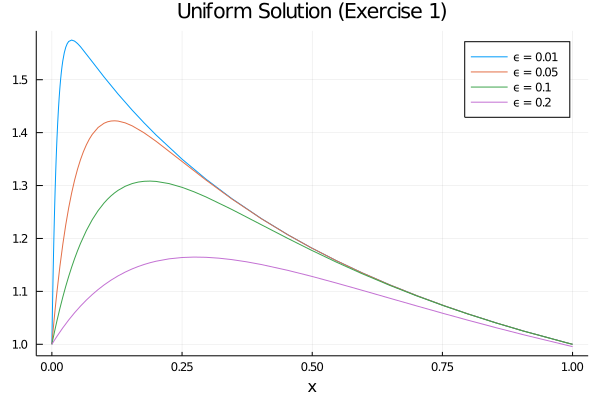
\includegraphics[width=0.8\linewidth]{figs/hw-5-exer-1.png}
    \caption{Plot of the uniform solution for exercise 1.}%
    \label{fig:figs/hw-5-exer-1}
\end{figure}


\end{sol}

\newpage

\begin{exer}

Consider the singular equation:
\begin{equation*}
    \epsilon \frac{d^{2} u}{dx^{2}} - x^{2} \frac{d u}{d x} - u = 0
\end{equation*}
with $u(0) = u(1) = 1$ and with $0 < \epsilon \ll 1$.
\begin{enumerate}[(a)]
    \item With the method of dominant balance, show that there are three distinguished limits: $\delta = \epsilon^{\frac{1}{2}}$, $\delta = \epsilon$, and  $\delta = 1$ (the outer problem). Write down each of the problems inthe various distinguished limits.
    \item Obtain the leading order uniform approximation (Hint: there are boundary layers ar $x = 0$ and $x= 1$).
    \item Plot the uniform solution for $\epsilon = 0.01$, $0.05$,  $0.1$,  $0.2$.
\end{enumerate}
\end{exer}

\begin{sol}
    (a) We begin by doing a perturbation expansion of the equations, so that we have equations
    \begin{align*}
        O(1): &\quad -x^{2} u_{0x} - u_{0} = 0\\
        O(\epsilon): &\quad - x^{2} u_{1x} - u_{1} = - u_{0xx}.
    \end{align*}
    As we do not know the location of the bounday layer, we will knot impose a specifc boundary condition. Rather, we show that our solution will be of the form 
    \begin{align*}
        u_{0}(x) = C e^{\frac{1}{x}},
    \end{align*}
    for some constant $C$ dependent on the boundary condition we impose. In order to analyze the inner problem, we'll introduce a stretching as before $\xi = x / \delta$ near $x=0$. This transforms our equations to 
    \begin{align*}
    \frac{\epsilon}{\delta^{2}} u_{\xi \xi} - \delta \xi^{2} u_{\xi} - u = 0\\
    \epsilon u_{\xi \xi} - \delta^{3} \xi^{2} u_{\xi} - \delta^{2} u = 0,
    \end{align*}
    The way to balance the first and last terms (given $O(\delta^{3})$ is much smaller than $O(\delta^{2})$) which gives a potential boundary layer of width $O(\epsilon^{1 / 2})$. 

    We now consider the distinguished limit near $x=1$, for which we define stetching $\xi = (1 - x) / \delta$. This transforms our equation as
    \begin{align*}
        \epsilon u_{\xi \xi} + \delta ( 1 - \delta \xi )^{2} u_{\xi} - \delta^{2} u = 0.
    \end{align*}
    In this case, the term $(1 - \delta \xi)^{2}$ is approximately one and the $\delta^{2}$ is much smaller than the rest, so we have 
\begin{equation*}
    \epsilon u_{\xi \xi} + \delta u_{\xi} = 0
\end{equation*}
and distinguished limit $\delta = \epsilon$. To construct the inner solution, we first begin with  $x = 0$ and $\xi = x / \epsilon^{1 / 2}$ as derived above which has leading order solution
\begin{align*}
    O(1): \quad u_{0\xi \xi} - u_{0} = 0, u_{0}(0) = 1.
\end{align*}
This gives solution $ u_{\text{in}0} = u_{0}(\xi) = e^{- \xi}$ as we require that $u_{0}$ is bounded in the $\xi \to \infty$ limit. Next for the second inner solution near $x = 1$ with stetching $\xi = (1 - x) / \epsilon$ as derived above, we have leading order equation
\begin{align*}
u_{0\xi \xi}  + u_{0\xi} = 0,\\
u_{0}(0) = 1, 
\end{align*}
which is solved as
\begin{align*}
    u_{\text{in}1}(\xi) = u_{0}(\xi) =  A e^{-\xi} + (1 - A).
\end{align*}
 
We'll now proceed to match our solutions
\begin{align*}
    u_{\text{out}} &= C e^{\frac{1}{x}}\\
    u_{\text{in}0} &= e^{- \xi}\\
    u_{\text{in}1} &=  A e^{-\xi} + (1 - A).
\end{align*}
Matching our equations results in the equations
\begin{align*}
    \lim_{x\to 0} u_{\text{out}} = \lim_{\xi \to \infty}  u_{\text{in}0}\\
    \lim_{x\to 1} u_{\text{out}} = \lim_{\xi \to \infty}  u_{\text{in}1}.
\end{align*}
Solving this shows that
\begin{align*}
    C \lim_{x\to 0} e^{\frac{1}{x}} &= \lim_{\xi \to \infty}  e^{-\xi} = 0\\
    0 = \lim_{x\to 1} C e^{\frac{1}{x}} &= \lim_{\xi \to \infty}  A e^{-\xi} + (1 - A) = 1 - A,
\end{align*}
so $C = 0$ and $A = 1$. We then write the uniform solution as 
\begin{align*}
    u_{\text{unif}} = \exp\left( - \frac{x}{\epsilon^{\frac{1}{2}}} \right) + \exp \left( - \frac{1- x}{\epsilon} \right),
\end{align*}
where we've included the proper definitions for various $\xi$.

(c) Solutions plotted below.

\newpage

\begin{figure}[h]
    \centering
    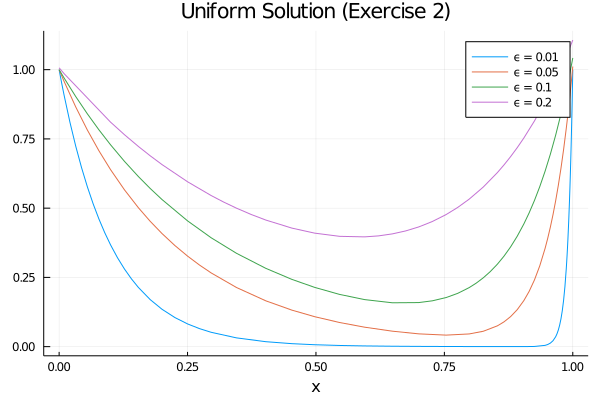
\includegraphics[width=0.8\linewidth]{figs/hw-5-exer-2.png}
    \caption{Plot of the uniform solution for exercise 2.}%
    \label{fig:figs/hw-5-exer-2}
\end{figure}
\end{sol}

\end{document}
